\documentclass[11pt,a4paper]{article}
\usepackage[T1]{fontenc}
\usepackage[utf8]{inputenc}
\usepackage{lmodern}
\usepackage[margin=2.5cm]{geometry}
\usepackage{amsmath,amssymb}
\usepackage{booktabs,tabularx}
\usepackage{graphicx}
\usepackage{xcolor}
\usepackage{listings}
\usepackage[hidelinks]{hyperref}

\graphicspath{{../outputs/}}

\definecolor{codebg}{HTML}{F6F6F4}
\definecolor{codekw}{HTML}{2A5DB0}
\definecolor{codecm}{HTML}{6B6A66}
\definecolor{codestr}{HTML}{8A4B12}
\lstdefinestyle{py}{
  language=Python, basicstyle=\ttfamily\footnotesize, backgroundcolor=\color{codebg},
  keywordstyle=\color{codekw}\bfseries, commentstyle=\color{codecm}\itshape,
  stringstyle=\color{codestr}, showstringspaces=false, breaklines=true,
  frame=single, rulecolor=\color{codebg}, columns=fullflexible, keepspaces=true,
  literate={-}{-}1
}
\lstset{style=py}
\newcommand{\code}[1]{\texttt{#1}}
% Include a scheduler step between the markers "# {name}" and "# {endname}".
\newcommand{\schedulerpart}[2]{\lstinputlisting[rangeprefix=\#\ \{, rangesuffix=\},
  linerange={#1-end#1}, includerangemarker=false, caption={#2}]{../model/scheduler.py}}
\newcommand{\eqfile}[1]{\lstinputlisting[caption={\code{\detokenize{equations/#1}}}]{../equations/#1}}
\newcommand{\marketfile}[1]{\lstinputlisting[caption={\code{\detokenize{markets/#1}}}]{../markets/#1}}
\newcommand{\rbar}{\bar r}
\newcommand{\qbar}{\bar q}

\title{Real competition in one industry: Shaikh against Okishio\\[0.3em]
\large An agent-based model, version 1 \\ M2 EPOG, MIP1 (Funalot \& Bassi)}
\author{The ABM group}
\date{\today}

\begin{document}
\maketitle
\tableofcontents

\section{Overview}

\paragraph{Question.} In an industry where cheaper techniques often need more capital per
unit of output, does market selection favour firms that equip new plants at the lowest unit
cost (Shaikh) or at the highest profit rate at the current price (Okishio)? How does the
answer depend on how often price wars occur and on how investment is financed?

\paragraph{The model.} One industry inside a given economy. The money wage is the
numéraire ($w = 1$), industry demand is exogenous, and the general rate of profit $\rbar$
is set outside the industry. Firms own plants of different vintages and techniques, post
prices, sell to a demand that moves towards cheaper firms, produce to order, scrap old or
obsolete plants, invest, enter and leave. Everything that is not the industry (buyers,
workers, suppliers, the lender and the owners) is one rest-of-economy account, so money is
conserved and the accounts are checked every period.

\paragraph{The neutrality rule.} Shaikh firms and Okishio firms differ only in the hurdle
$h$ they use to choose techniques, in investment, replacement and entry. Pricing, demand,
production and accounts, physical scrapping and exit treat both types the same. In the code
the type label is used only to look up the hurdle rule (\code{equations/hurdle.py}) and to
pass it on to entrants; the label-swap tests
run the model with the labels swapped everywhere except the hurdle and require identical
trajectories.

\paragraph{Version 2.} Each mechanism keeps the starting rule of its brief behind a switch
and runs by default on the rules agreed on 6 November 2026: plants of fixed size $S = 20$
with no maximum age, scrapped after two periods with the price below their unit cost or
two periods idle; pricing without anchor or war trigger, where cuts come from cost edges;
investment of all retained earnings in whole plants, with no borrowing, and one
Marx-biased design offered at each investment; bankruptcy when cash runs out; entrants
pricing by the common rule; $\rbar = 0.05$. The pricing rule (cost-edge undercutting, or
the group's leader-follow rule under which every firm cuts whenever capacity is not short)
and the technical-change rule (designs drawn by category, or from an innovation set) are
the model's two most sensitive parts: both are switches, their defaults are frozen since
7 November 2026, and a sensitivity analysis decides whether each becomes a fixed choice or
a treatment (\code{docs/design/review-v2.md}). Every further choice is listed in
section~\ref{sec:choices} and in \code{docs/design/choices.md}, which also records the
version 1 values. The test industry is Shaikh's three plants (2016, Tables 7.10--7.11):

\begin{center}
\begin{tabular}{lrrrrrr}
\toprule
Plant & Normal output & Capital & $\kappa$ & $uc$ & $ucs$ & $r$ at $p = 100$ \\
\midrule
C  & 120 & 16{,}500 & 137.50 & 78 & 64.25 & 16.00\,\% \\
D1 & 130 & 18{,}500 & 142.31 & 76 & 61.77 & 16.86\,\% \\
D2 & 133 & 21{,}000 & 157.89 & 75 & 59.21 & 15.83\,\% \\
\bottomrule
\end{tabular}
\end{center}

Each plant is given to one Shaikh and one Okishio firm (six firms, identical within each
pair) and split into plants of 20; demand is $680 = (340/383)\times 766$, $\delta = 0.10$,
$\rbar = 0.05$ (0.16 in version 1) and $u_{\max} = 1.2$.

\paragraph{Baseline run.} Figures~\ref{fig:prices}--\ref{fig:firms} show the baseline
(seed 42, 200 periods, version 2 defaults). The D1 and D2 firms undercut C from $t = 0$
and the opening war takes prices from 100 to 73 by $t = 20$; afterwards prices follow unit
costs down as designs are adopted (Shaikh firms' unit cost 46 at $t = 199$, price 49),
with a cut in 126 of 200 periods and 50 periods of excess demand after scrapping. With
$\rbar = 0.05$ the rate on new plants is above $\rbar$ almost every period: 43 firms enter
and 42 leave, nearly all by falling below 1\,\% of the market. Okishio firms fall below
1\,\% of the market at $t = 75$ and entrants that switch rule bring them back to 7\,\% by
$t = 199$; 7 firms remain. Over seeds 1--20 Shaikh firms win 16 runs. Whether they win
through prices or through accumulation is what the collector's decomposition
(section~\ref{sec:accounts}, \code{docs/design/collector.md}) is for; until the
sensitivity analysis has run, this is a baseline, not a result.

\begin{figure}[p]
\centering
\includegraphics[width=0.85\textwidth]{prices.png}
\caption{Posted prices: sales-weighted mean and range.}\label{fig:prices}
\vspace{1em}
\includegraphics[width=0.85\textwidth]{shares_by_type.png}
\caption{Market shares by type.}\label{fig:shares}
\end{figure}

\begin{figure}[p]
\centering
\includegraphics[width=\textwidth]{capacity.png}
\caption{Normal capacity of the plants that produced, by technique and by type.}\label{fig:capacity}
\vspace{1em}
\includegraphics[width=0.85\textwidth]{profit_rates.png}
\caption{Profit rates by type and the entry trigger $r^{new}$.}\label{fig:rates}
\end{figure}

\begin{figure}[t]
\centering
\includegraphics[width=0.85\textwidth]{n_firms.png}
\caption{Number of firms by type.}\label{fig:firms}
\end{figure}

\section{Notation}

Python names are those used in the code (attributes, function arguments). Parameters are
upper case in \code{parameters.py} (\code{DELTA}, \code{RBAR}, \code{RHO}, \ldots) and passed
to the equations under the lower-case names below.

\begin{center}
\begin{tabularx}{\textwidth}{llX}
\toprule
Symbol & Python name & Meaning \\
\midrule
$p_i$ & \code{price} & posted price of firm $i$ \\
$D_t$ & \code{demand} & industry demand, units per period (exogenous) \\
$f_i$ & \code{share} & market share \\
$x_i$ & \code{sales} & units sold, equal to output (no inventory) \\
$\qbar_i$ & \code{capacity} & normal output of the firm's plants; output can stretch to $u_{\max}\qbar_i$ \\
$u_i$ & \code{util} & utilisation $x_i/\qbar_i$ \\
$ucs_v$ & \code{ucs} & unit operating cost of plant $v$ \\
$\kappa_v$ & \code{kappa} & capital per unit of normal output \\
$\delta$ & \code{delta} & depreciation rate, $1/T$ \\
$uc_v$ & \code{uc} & unit cost $ucs_v + \delta\kappa_v$ \\
$h_i$ & \code{hurdle} & 0 for Shaikh firms; the best profit rate on offer at the firm's price for Okishio firms \\
$\rbar$ & \code{rbar} & general rate of profit \\
$M_i, B_i$ & \code{cash}, \code{debt} & balance sheet \\
$\Pi_i$ & \code{profit} & profit after depreciation and interest \\
$NW_i$ & \code{net\_worth} & cash plus book value of plants, minus debt \\
$\rho$ & \code{rho} & interest rate on debt \\
$r^{new}$ & \code{r\_new} & profit rate on plants built in the last $k$ periods \\
\midrule
$S$ & \code{PLANT\_SIZE} & capacity of every plant (version 2) \\
$RE_i$ & \code{retained\_earnings} & profit less dividends since birth, less spending on plants \\
$\mathit{wear}_v$ & \code{wear} & output so far in periods of normal output, $\sum_t x_{v,t}/\qbar_v$ \\
$a, b$ & \code{draw\_design} & a design's proportional fall in $ucs$ and rise in $\kappa$ \\
$q$ & \code{TECH\_CONFLICT} & share of designs drawn in the conflict zone \\
$z$, floor markup & \code{LEADER\_RISE}, \code{FLOOR\_MARKUP} & leader-follow rule: rise after a shortage; markup of the floor on average unit cost \\
\bottomrule
\end{tabularx}
\end{center}

Two symbols of the brief are used twice there and are renamed in the code: the plant life
$T = 1/\delta$ is \code{PLANT\_LIFE} and the length of the price-war trigger is
\code{WAR\_PERIODS}; the price band $b$ is \code{PRICE\_BAND}. The mutation rate of the
entry brief is $m$; the leader-follow floor markup is written out in words to keep $m$ for
it.

\section{Order of events}

\code{model/scheduler.py} runs one period; each step sees only what earlier steps produced.

\begin{enumerate}
\item \textbf{Start.} Plants bought last period arrive; flows are reset.
\item \textbf{Pricing.} Firms post $p_i$ from last period's prices, utilisation and leader.
\item \textbf{Demand.} Shares from prices, demand allocated within capacity, sales and utilisation.
\item \textbf{Production and accounts.} Plants run in merit order; profits, dividends, cash and debt.
\item \textbf{Scrapping.} Hurdles are updated; plants retire by age or obsolescence; replacement.
\item \textbf{Investment.} Desired capacity, technique chosen with $h$, finance; plants arrive next period.
\item \textbf{Entry and exit,} then the collector and the stock-flow check.
\end{enumerate}

\begin{figure}[h]
\centering
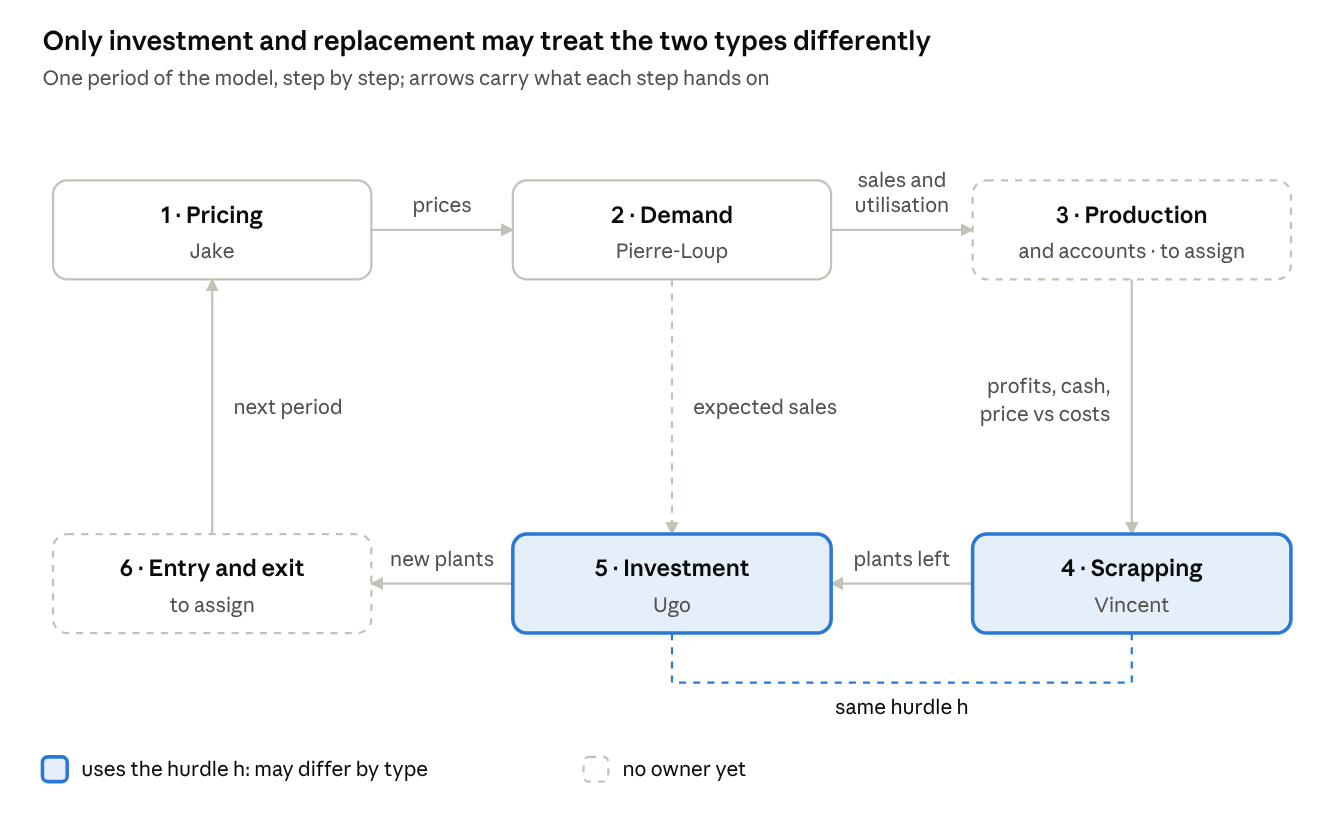
\includegraphics[width=0.7\textwidth]{../docs/design/img/2026-10-16_ABM-Project_mechanism-briefs_one-period.png}
\caption{One period: six steps, one shared hurdle (from the briefs).}
\end{figure}

\schedulerpart{period}{\code{model/scheduler.py}: one period}

\section{Pricing (Jake)}\label{sec:pricing}

Pricing is where real competition happens: the low-cost firm cuts its price, followers
match, and cuts stop at cost (Shaikh 2016, Table 7.3). Version 2 has no anchor and no war
trigger: a firm cuts only when it is cheaper than a rival at the lowest price, so price wars
come from cost differences, and technical change is what renews them. The group's
leader-follow rule, in which every firm cuts whenever capacity is not short, is the other
end of the price-war treatment; the two rules are the model's most sensitive switch, and
the sensitivity analysis decides whether one is fixed or both are kept as a treatment
(\code{docs/design/review-v2.md}).

\paragraph{Rule} (\code{PRICING\_RULE = "real\_competition"}). With
$R_{i,t} = \min_{j\neq i} p_{j,t-1}$ the lowest rival price,
$uc_i = \min_{v}(ucs_v + \delta\kappa_v)$ the unit cost of firm $i$'s best plant, $E_{t-1}$
last period's demand above normal capacity and $D_{t-1}$ last period's demand,
\[
p_{i,t} =
\begin{cases}
\min\{\, p_{j,t-1} : p_{j,t-1} > p_{i,t-1} \,\} & \text{if } E_{t-1} > 0
  \text{ and some rival priced higher}, \\
(1 + \eta\, E_{t-1}/D_{t-1})\, p_{i,t-1} & \text{if } E_{t-1} > 0
  \text{ and no rival priced higher}, \\
\min\{\, p_{i,t-1},\ (1-c)\,R_{i,t} \,\} & \text{if } u_{i,t-1} < 1 \text{ and }
  uc_i < \min\{(1-c)R_{i,t},\ \max_{j:\,p_{j,t-1}=R_{i,t}} uc_j\}, \\
\max\{\, \min\{p_{i,t-1}, R_{i,t}\},\ uc_i \,\} & \text{otherwise,}
\end{cases}
\]
with $c = 0.02$ and $\eta = 0.5$. In words: under excess demand, move up to the next higher
price, and the firm at the top raises it; with spare capacity and a cost edge over a rival
at the lowest price, undercut it; otherwise follow the lowest price, never below one's own
unit cost. The leader is whoever posts the lowest price: it is not assigned, and the
lowest-cost firm leads in 187 of 200 periods with the version 1 plants and accelerator
(seeds 1--10, $\rbar = 0.16$), in 58 under the version 2 defaults.

\paragraph{Why each detail.} $R$ excludes the firm itself, or a lone leader would undercut
itself every period. A cut never raises the firm's price. The edge is over \emph{a} rival at
$R$, so an identical twin at $R$ does not block the cut. The top-priced firm must be able to
raise, or prices could only fall. Excess demand is measured against normal capacity
(\code{EXCESS\_DEMAND = "normal\_capacity"}): against all output with overtime
(\code{"unserved"}), the 20\,\% overtime margin absorbs every shortage and prices end at
C's unit cost, 78.5. The floor is the firm's own unit cost; \code{PRICE\_FLOOR =
"operating\_cost"} uses the version 1 floor ($ucs$, Shaikh 2016, p.~316), with which
followers match the leader all the way down.

\paragraph{What moves the price in version 2.} Under the version 2 defaults the price does
not get stuck: retained earnings keep buying plants, idle scrapping keeps capacity near
demand, and each adopted design gives its owner a cost edge that starts a cut (a cut in 126
of 200 periods at seed 42). Shortages come from scrapping, not from under-investment. With
the version 1 plants and accelerator ($\rbar = 0.16$) the war of t = 0--19 drove prices to
78.5, a shortage at t = 20 lifted them to 89.9, and then nothing moved: capacity was rebuilt
to last sales and no firm could cut. The scratch test with profit-sensitive investment,
desired capacity $x_{t-1}(1+\beta(r_i-\rbar)/\rbar)$ with $\beta = 0.25$, under which the
price gravitates around 99 and the profit rate around 15.7\,\%
(\code{docs/design/choices.md}), remains the proposal for the accelerator arm of the
finance treatment.

\paragraph{Version 1} (\code{PRICING\_RULE = "anchor"}), kept for comparison. Firms move
towards an anchor, stay within a band of the leader, and cut collectively after a run of low
utilisation:
\begin{gather*}
p^N_i = uc_i + \rbar\,\kappa_i \quad\text{(capacity-weighted over the firm's plants)}, \qquad
p_{i,t} = \max\{\, ucs_i,\ \tilde p_{i,t} \,\}, \\
\tilde p_{i,t} =
\begin{cases}
(1-c)\, p_{i,t-1} & \text{if } u_{i,t-k} < u^{war},\ k = 1,\dots,T_{war}, \\
\min\{\, p_{i,t-1} + \lambda\,(p^{N}_i - p_{i,t-1}),\ (1+b)\, p^{lead}_{t-1} \,\} & \text{otherwise,}
\end{cases}
\end{gather*}
with $u^{war} = 0.95$, $T_{war} = 2$, $b = 0.025$, $\lambda = 0.25$.
\code{PRICING\_ANCHOR = "markup"} uses $(1+\mu)uc_i$; \code{"leader"} gives every firm the
target-return price of last period's leader. Over seeds 1--10 the final share of Shaikh
firms is 0.12 under each firm's own target return, 0.82 under the markup and 0.51 under the
leader's anchor: the anchor decides the winner.

\paragraph{Alternative: follow and undercut the leader} (\code{PRICING\_RULE =
"leader\_follow"}, proposed from the group's notebook). With $p^{lead}_{t-1}$ the lowest price
posted last period and a floor at a markup on average unit cost,
\begin{gather*}
\underline p_{i} = (1+m)\,\overline{uc}_i \quad\text{(capacity-weighted over the firm's plants)}, \\
p_{i,t} =
\begin{cases}
\min\{(1+z)\,p_{i,t-1},\ \bar m\,\underline p_{i}\} & \text{if } i \text{ is the only firm}, \\
(1+z)\,p^{lead}_{t-1} & \text{after excess demand}, \\
\max\{\underline p_{i},\ (1-c)\,p^{lead}_{t-1}\} & \text{otherwise},
\end{cases}
\end{gather*}
with $c = 0.02$, $m = 0.20$, $z = 0.03$, $\bar m = 3$ (\code{PRICE\_CUT}, \code{FLOOR\_MARKUP},
\code{LEADER\_RISE}, \code{MONOPOLY\_CAP}) and excess demand measured as in the default rule.
Every firm cuts whenever capacity is not short, so prices fall each period to the floors, and
the firm with the lowest floor sets the price. Unlike the notebook, $c$, $m$ and $z$ are the
same for every firm rather than drawn at random for each, so identical firms stay identical
and the label swap holds. Over seeds 1--10 under the version 2 defaults the leader is the
lowest-cost firm in 195 of 200 periods (58 under the default rule) and the final share of
Shaikh firms is 0.55 (0.81). Two points of the rule are open for the sensitivity analysis:
the floor, a 20\,\% markup on the firm's average unit cost under which no plant ever sells
below its unit cost and the Okishio hurdle never reaches zero (the version 2 default stops
cuts at the best plant's unit cost, version 1 at operating cost); and the shortage branch,
under which every firm posts $(1+z)\,p^{lead}_{t-1}$, so that a firm priced above that
lowers its price in a shortage.

\paragraph{Tests} (\code{tests/test\_pricing.py}): the rule's branches one by one (cut with an
edge and spare capacity; no cut without either, nor against an identical twin; a cut never
raises a price; the leader does not undercut itself; follow down to the floor and no further;
excess demand moves prices up); no price below the floor and no rise without excess demand
over 2\,000 random cases; identical firms with spare capacity never start a war; on the test
industry D2 cuts first, the others follow to their unit costs, and excess demand raises every
price; with the operating-cost floor the war ends on one price; the label swap holds under each
switch. Version 1 keeps its tests (1)--(4) and the leader-anchor tests. The leader-follow
rule: its branches one by one, prices falling to $1.2\,uc$ on the test industry, identical
firms posting identical prices, and the label swap.

\subsection*{Code}
\eqfile{anchor_price.py}
\eqfile{price_floor.py}
\eqfile{price_war.py}
\eqfile{real_competition_price.py}
\eqfile{leader_follow_price.py}
\eqfile{posted_price.py}
\schedulerpart{pricing}{\code{model/scheduler.py}: step 1}

\section{Demand (Pierre-Loup)}\label{sec:demand}

Demand allocation is the selection environment: it sets how fast a price advantage becomes
market share, and so whether a price war pays. The selection intensity $\chi$ may be the
most important parameter of the project. With strong selection a small price cut moves
customers fast, price wars pay and the unit-cost rule gains; with weak selection shares
barely move and firms with higher profit rates win by accumulating faster. Selection is weak
in the data (Dosi et al.\ 2015; Foster, Haltiwanger \& Syverson 2008), so results must be
reported at weak selection too.

The course's K+S formula uses a negative competitiveness; divided by a negative mean, the
update would send customers to the dearer firm. Version 1 uses the positive
competitiveness $E = 1/p$. Industry demand is insensitive to the industry price, so price
wars only move customers between firms.

\paragraph{Starting rule.}
\[
E_{i,t} = \frac{1}{p_{i,t}}, \qquad \bar E_t = \sum_j f_{j,t-1}\, E_{j,t}, \qquad
f_{i,t} = f_{i,t-1}\left(1 + \chi\, \frac{E_{i,t} - \bar E_t}{\bar E_t}\right), \quad \chi = 1.
\]
Shares cut below zero are set to zero and the others renormalised. A firm sells
\[
x_{i,t} = \min\{f_{i,t} D_t,\ \text{output it offers at } p_{i,t}\},
\]
where the output
offered is the capacity of the plants whose operating cost the price covers, up to
$u_{\max}\qbar_i$. The overflow goes to the cheapest firms with spare capacity (tied firms
share it in proportion to spare capacity); each firm's unmet demand and the demand nobody
can serve are recorded. Utilisation is $u_{i,t} = x_{i,t}/\qbar_i$. At $\chi = 1$, a small
firm 2\,\% cheaper than average grows its share by about 2\,\% a period.

The alternative \code{DEMAND\_FORM = "logit"} sets $f_{i,t} \propto f_{i,t-1}\, p_{i,t}^{-\eta}$,
which never produces negative shares; with $\eta = 1$ it responds like $\chi = 1$ to small
gaps.

\paragraph{Tests} (\code{tests/test\_demand.py}): shares non-negative and summing to one;
equal prices leave shares unchanged; a firm 2\,\% cheaper gains share at the rate $\chi$
predicts; overflow goes to others and no unit is sold twice; ties are shared pro rata;
swapping the type labels changes nothing.

\subsection*{Code}
\eqfile{competitiveness.py}
\eqfile{market_shares.py}
\eqfile{offered_capacity.py}
\marketfile{goods_market.py}
\schedulerpart{demand}{\code{model/scheduler.py}: step 2}

\section{Production and accounts (to assign)}\label{sec:accounts}

Production and accounts turn sales into output, costs, profits and balance sheets; every
other mechanism reads them, and this is where the model checks its stock-flow consistency.

\paragraph{The trap: the accounts define the profit rate every rule compares.} Profit gross
of depreciation puts every rate $\delta$ above the net rate $(p - uc)/\kappa$ that $\rbar$
measures; dividing by book value makes the oldest plants look the best. One definition is
used everywhere: profit net of depreciation and interest, over capital at purchase cost.
Book values serve only for net worth.

\paragraph{Starting rule.} Firms produce to order: output equals sales, and plants run in
merit order, lowest operating cost first. Output above normal capacity costs a premium of
10\,\% on $ucs$ (\code{OVERTIME\_PREMIUM}), the same for both types.
\begin{align*}
\Pi_{i,t} &= (p_{i,t} - ucs_i)\,x_{i,t} - \text{premium} - \textstyle\sum_v \delta\,\kappa_v\,\qbar_v - \rho\,B_{i,t-1},
  \qquad r_{i,t} = \frac{\Pi_{i,t}}{\sum_v \kappa_v\,\qbar_v}, \\
M_{i,t} &= M_{i,t-1} + \Pi_{i,t} + \textstyle\sum_v \delta\,\kappa_v\,\qbar_v - \mathit{Div}_{i,t}
  - \kappa_{j^*}\,I_{i,t} + \Delta B_{i,t}, \qquad \mathit{Div}_{i,t} = d\,\max\{0, \Pi_{i,t}\}, \\
NW_{i,t} &= M_{i,t} + K^{b}_{i,t} - B_{i,t},
\end{align*}
with $\rho = 0.05 < \rbar$ and $d = 0.5$ for both types. Book values fall in a straight line
over $T$ periods; a plant retired early leaves its book value as a write-off, which lowers
net worth while no cash moves. Firms repay 10\,\% of their debt a period from cash. In version 1 a
negative cash balance is covered by an overdraft loan; in version 2
(\code{CASH\_SHORTFALL = "bankruptcy"}, the default) it stays as bills the firm could not
pay, and the firm goes bankrupt at the end of the period (section~\ref{sec:entry}). Since a
firm sells only what plants whose $ucs$ the price covers can make, and dividends come out of
positive profit, cash runs out only when interest exceeds the operating margin.

\paragraph{Alternative: depreciation by use.} With \code{DEPRECIATION = "use"} (the default
is \code{"time"}) a plant depreciates with what it produces, $\delta\,\kappa_v\,x_{v,t}$
(overtime included), instead of $\delta\,\kappa_v\,\qbar_v$ a period, until its book value is
zero. Its purchase cost is then spread over a lifetime output of $\qbar_v/\delta$. At normal
output both rules charge the same, and the capital charge per unit of output is
$\delta\kappa_v$ in both, so $uc = ucs + \delta\kappa$, and with it the hurdle, the
technique choice, replacement and the scrap cost, are unchanged. What changes is the cost of
idle capacity: an idle plant does not depreciate, so a firm at low utilisation reports a
higher profit, and a plant scrapped while idle leaves a larger write-off. Under this rule
\code{PLANT\_LIFE} counts periods of normal output rather than age: a plant leaves once it
has produced \code{PLANT\_LIFE}$\times\qbar_v$, which with \code{PLANT\_LIFE} $= 1/\delta$ is
when it is fully depreciated. The rule is the same for both types.

\paragraph{Closure.} Wages and materials, plant purchases, interest, dividends, loans,
equity and the industry's demand all go through one rest-of-economy account. Every payment
goes through \code{markets/payments.pay}, which records the transaction-flow matrix. At the
end of each period the scheduler asserts that money is conserved, that firms' debt equals
the loans of the rest of the economy, that each firm's net worth moved by
$\Pi - \mathit{Div} - \text{write-offs}$ (plus equity at entry), and that every row and
column of the flow matrix adds up.

\paragraph{Tests} (\code{tests/test\_accounts.py}, \code{tests/test\_production.py}): at
normal output with no debt $r_i = (p - uc)/\kappa$, i.e.\ 16.00\,\%, 16.86\,\% and 15.83\,\%
at $p = 100$; the net-worth identity; the flow matrix sums to zero; depreciation charges add
up to the purchase cost and book value is zero at age $T$; a firm without sales loses
exactly depreciation plus interest; merit order, overtime and ties; label swap.

\subsection*{Code}
\eqfile{merit_order.py}
\eqfile{operating_cost.py}
\eqfile{depreciation.py}
\eqfile{interest_payment.py}
\eqfile{firm_profit.py}
\eqfile{profit_rate.py}
\eqfile{plant_profit.py}
\eqfile{dividends.py}
\eqfile{debt_repayment.py}
\marketfile{payments.py}
\marketfile{credit_market.py}
\schedulerpart{accounts}{\code{model/scheduler.py}: step 3}

\section{Scrapping (Vincent)}\label{sec:scrapping}

Scrapping decides how long old plants survive: it sets the spread of vintages behind
unequal margins, the speed at which a new technique spreads, and which plant sets the floor
of a price war. Three decisions are kept apart in the code: \emph{run or idle} (production,
in merit order), \emph{retire} (age or obsolescence, identical for both types) and
\emph{replace} (a second choice of technique, where the types differ through $h$).

\paragraph{The trap: replacement is a second choice of technique.} With the hurdle $h$,
replacing plant $v$ by technique $n$ pays when
\[
ucs_v > ucs_n + (\delta + h)\,\kappa_n .
\]
Shaikh firms ($h = 0$) replace earlier, which gives them younger capital and faster
diffusion; Okishio firms keep old plants longer. Retirement is therefore identical for both
types, and only replacement uses $h$, the same $h$ as investment.

\paragraph{Starting rule.} A plant retires at age $T = 1/\delta = 10$, or once its owner's
price has stayed below its $ucs$ for $N = 4$ periods (its quasi-rent is negative, Salter
1966). Replacement is on in version 1: the firm compares each working plant with the
technique its own hurdle picks, and replaces it if the inequality holds and the firm can pay
(cash, then debt up to the cap). Scrap value is zero; remaining book value is written off.
Depreciation is accounting only. When a firm's last plant retires, its lifetime profit rate
decides non-renewal (section~\ref{sec:entry}).

\paragraph{Tests} (\code{tests/test\_scrapping.py}): a plant reaching age $T$ leaves; a plant
whose $ucs$ stays above the price for $N$ periods leaves; an old plant with $ucs = 80$
facing a technique with $ucs = 60$, $\kappa = 150$: a Shaikh firm replaces it
($75 < 80$), an Okishio firm at $h = 16\,\%$ keeps it ($99 > 80$); on the test industry no
working plant is replaced; capacity after scrapping equals capacity before minus retired
plants.

\subsection*{Code}
\eqfile{retirement.py}
\eqfile{replacement.py}
\eqfile{lifetime_profit_rate.py}
\schedulerpart{scrapping}{\code{model/scheduler.py}: step 4}

\section{Investment (Ugo)}\label{sec:investment}

Investment carries the rule under test. It makes three decisions: how much capacity to add,
which technique the new plants embody, and how to pay for them. Only the second may differ
between the two types.

\paragraph{The trap: quantity and finance can settle the contest before the technique rule
does.} If firms invest all their cash, capacity grows with profits and the firms with the
higher profit rate at the going price, the Okishio firms, grow faster. Investment also
creates the excess capacity that starts price wars, which favour Shaikh firms. The volume
rule sets the balance between the two selection channels, so it is identical for both types.

\paragraph{Version 1 rule.}
\[
\qbar^{\,d}_{i,t} = (1+g)\, x_{i,t-1}, \qquad
I_{i,t} = \max\{0,\ \qbar^{\,d}_{i,t} - \qbar_{i,t}\}, \qquad
j^{*} = \arg\min_{j}\, \big[(1 + h_i\tau)\, ucs_j + (\delta + h_i)\, \kappa_j\big],
\]
with $g = 0$, $\tau = 0$, $\qbar_{i,t}$ the capacity left after scrapping plus plants on
order, and the menu C, D1, D2. Shaikh firms use $h = 0$, which picks the lowest unit cost;
Okishio firms use the best profit rate on the menu at their own current price, floored at
zero, which picks the highest profit rate at that price. New plants arrive next period and
are paid from cash, then debt up to twice the period's sales revenue; investment is scaled
down when it cannot be financed.

\paragraph{Version 2 rules (the defaults).} \code{PLANT\_SIZE} $= S$ gives every plant the
capacity $S$, including the initial plants (split into the nearest number of plants) and
entrants'. \code{INVESTMENT\_RULE = "retained\_earnings"} replaces the accelerator: whatever
the demand, firm $i$ buys as many plants of the technique $j^*$ as its retained earnings pay
for,
\[
I_{i,t} = S \left\lfloor \frac{\min\{RE_{i,t},\ M_{i,t}\}}{\kappa_{j^*} S} \right\rfloor,
\qquad RE_{i,t} = RE_{i,t-1} + \Pi_{i,t} - \mathit{Div}_{i,t} - \kappa_{j^*} I_{i,t-1},
\]
with $\Pi$ profit after depreciation and interest, $M$ cash, and $I$ all spending on plants,
replacement included. \code{BORROWING = False} removes borrowing for plants everywhere:
investment, under either rule, and replacement are paid from cash only, and the debt cap no
longer binds anything. With \code{CASH\_SHORTFALL = "bankruptcy"} there is no overdraft
either (section~\ref{sec:accounts}). Without a demand condition,
capacity is bounded only by scrapping: without \code{IDLE\_SCRAPPING} it grows without limit
(section~\ref{sec:scrapping}, \code{docs/design/choices.md}).

\paragraph{The two channels.} The retained-earnings rule is the accumulation channel of
the brief's trap, chosen deliberately: capacity grows with each type's profits, and the
firms with the higher profit rate at the going price grow faster. The price channel runs
alongside through market shares. The decomposition of each type's capacity share into net
investment, entry and exit, and of its sales share into price-driven, entry-exit and
rationing terms (\code{docs/design/collector-brief.md}, \S4.2--4.3;
\code{analysis/indicators.py}), is reported with every result. The version 1 accelerator
with borrowing (\code{INVESTMENT\_RULE = "accelerator"}, \code{BORROWING = True}) is the
other arm of the finance treatment.

\paragraph{Technical change (version 2 default).} With \code{TECH\_DRAWS = True}, the default (\code{TECH\_CONFLICT} $= q = 0.5$), a firm that invests is
offered one new design $n$, drawn relative to the technique $o$ it would otherwise build and
judged at its own price $p$. Every design is Marx-biased: operating cost falls by a share
$a \le$ \code{TECH\_STEP} and capital per unit rises by a share $b$,
\[
ucs_n = (1-a)\,ucs_o, \qquad \kappa_n = (1+b)\,\kappa_o .
\]
Unit cost falls if $b < b_S = a\,ucs_o/(\delta\kappa_o)$, and the profit rate at $p$ rises if
$b < b_O = a\,ucs_o/(\delta\kappa_o + p - uc_o)$. With probability \code{TECH\_CONFLICT} the
design lies in the conflict zone $b_O \le b < b_S$, which only the unit-cost rule adopts;
otherwise $0 < b < b_O$ and both rules adopt it. The conflict zone vanishes as the margin
$p - uc_o$ falls to zero, where the two rules coincide. The firm adopts $n$ if
$ucs_n + (\delta + h_i)\kappa_n < ucs_o + (\delta + h_i)\kappa_o$, the same comparison as the
technique choice, and keeps it among the techniques it knows; if not, it still invests, in
$o$, so a rejected design never costs a firm capacity. Each draw is logged (its zone, its
unit cost, whether it was adopted, and the order that builds it).

This rule has limits that keep it from carrying the contest on its own: the conflict share
$q$ is set by a coin flip rather than produced by an innovation set, so a price war cannot
close the conflict zone except at zero margin; no design is ever rejected by a unit-cost
firm; there are no capital-saving designs; the draw reads the firm's price; a firm that
invests more often is offered more designs; and designs are private to the adopter but
public to entrants. The innovation set below answers them; it is the second arm of the
switch \code{TECH\_CHANGE}, the default (\code{"categories"}) staying as it is until the
sensitivity analysis.

\paragraph{Innovation set} (\code{TECH\_CHANGE = "innovation\_set"},
\code{equations/innovation\_set.py}). A design $n$ is drawn relative to a reference
technique $o$ with nothing read from the firm but $o$:
\[
ucs_n = (1-a)\,ucs_o, \qquad \kappa_n = (1+b)\,\kappa_o, \qquad
a = u\,\text{\code{TECH\_STEP}}, \qquad b = k\,a, \qquad k = m\,e^{\sigma z},
\]
with $u$ uniform on $(0, 1]$ and $z$ standard normal (\code{TECH\_SET = "marx"}: every
design saves labour and uses capital). $k$ is the capital per unit given up per unit of
operating cost saved, log-normal around the median $m$ (\code{TECH\_BIAS} $= 1.5$, the
treatment) with spread $\sigma$ (\code{TECH\_BIAS\_SPREAD} $= 0.8$). The adoption
inequality is unchanged, so in terms of $k$ the unit-cost rule adopts if
$k < k_S = ucs_o/(\delta\kappa_o)$ and the profit-rate rule at price $p$ if
$k < k_O(p) = ucs_o/(\delta\kappa_o + \max\{0, p - uc_o\})$: the zones (both adopt,
conflict, both reject) are outcomes of the draw and of the price, and a price war closes
the conflict zone. For C at $p = 100$, $k_O = 1.80$ and $k_S = 4.67$; at the median bias of
the Penn World Table ($m = 0.53$) the rules agree on 94\,\% of draws at normal prices and
on all of them in a war; at $m = 1.5$ to $3$ the conflict share is 20 to 45\,\% at normal
prices and zero in a war (\code{docs/design/review-v2.md}, section 4, zone shares). The
neutral set (\code{TECH\_SET = "neutral"}) draws the direction uniformly on the circle in
the plane $(\Delta ucs/ucs, \Delta\kappa/\kappa)$ with size $u\,$\code{TECH\_STEP}:
capital-saving and dearer designs appear, the second wedge (only the profit-rate rule
adopts) with them, and realised Marx bias becomes an outcome, read from the
capacity-weighted $ucs$ and $\kappa$ of each type in the \code{groups} table. Three further
switches: the reference is the firm's best known technique (\code{TECH\_REFERENCE = "own"})
or the industry's lowest-unit-cost technique in use (\code{"frontier"}); designs are
offered once per firm and period with probability \code{TECH\_DRAW\_RATE} $= 0.2$ whether
or not the firm invests (\code{TECH\_DRAW\_TIMING = "period"}; an adopted design is built at
the next investment) or at each investment as in the categories rule
(\code{"investment"}); a design becomes known to every firm \code{IMITATION\_LAG} $= 2$
periods after its first plant produces (\code{TECH\_DIFFUSION = "public"}), or stays with
its adopter and later entrants (\code{"private"}). Every draw is logged with its zone at
the firm's price; the label swap holds under each switch.

\paragraph{Tests} (\code{tests/test\_investment.py}): at $p = 100$ Shaikh firms build D2 and
Okishio firms D1, and with only C and D2 on offer Okishio firms keep C; on random menus the
argmin with $h$ equal to the best profit rate picks the same technique as maximising the
profit rate directly; with constant demand and no scrapping, investment stops once capacity
meets expected sales; borrowing for plants never takes debt above its cap; two firms of
different types with the same sales add the same capacity. For the switches: whole plants
for a capacity; retained earnings buy whole plants and never borrow; with \code{BORROWING = False} no firm
borrows for plants over a run, under either investment rule, and replacement waits for cash; every plant, entrants'
included, has the fixed size; every design uses more capital and less operating cost and is
adopted exactly by the rules its category names; at zero margin both rules adopt a conflict
design; operating costs stay positive over a long run; a rejected design still leaves the
firm investing in its best known technique, an adopted one is built and kept; the label
swap holds with draws.

\subsection*{Code}
\eqfile{hurdle.py}
\eqfile{technique_choice.py}
\eqfile{desired_capacity.py}
\eqfile{investment.py}
\eqfile{retained_earnings_investment.py}
\eqfile{plant_number.py}
\eqfile{new_technique.py}
\eqfile{innovation_set.py}
\eqfile{borrowing_capacity.py}
\marketfile{plant_market.py}
\schedulerpart{investment}{\code{model/scheduler.py}: step 5}

\section{Entry and exit (to assign)}\label{sec:entry}

Entry and exit move capital between the industry and the rest of the economy, and decide
which rule the population carries in the long run. For Shaikh, the entry and exit of
capital ``serve to equalize profit rates on new investment'' (2016, p.~264). Entry is
decisive: no price lets D2 earn the normal rate and keep C out.

\paragraph{The trap: entry is a third choice of technique.} If every entrant followed one
rule, the contest would be settled by construction. The decision is split in two: a trigger
both types share, then a rule the entrant inherits and uses to pick its plant. Exit has its
own trap: if capital leaves only through bankruptcy, a firm earning far below $\rbar$ stays
as long as its net worth is positive, so non-renewal is a second channel.

\paragraph{Starting rule.}
\begin{gather*}
\Pr(\text{entry}_t) = \min\left\{1,\ \theta\,\frac{\max(0,\ r^{new}_t - \rbar)}{\rbar}\right\}, \qquad
h_e = h_j \ \text{ with } \Pr(j) = f_{j,t}, \\
\text{exit if } NW_{i,t} < 0, \ \text{ or } f_{i,t} < f_{\min}, \ \text{ or non-renewal}.
\end{gather*}
$r^{new}_t$ is the realised profit rate this period of the plants that came into operation
in the last $k = 5$ periods, capacity-weighted, and $\theta = 5$; at most one firm enters a
period. With $\rbar = 0.05$ and $\theta = 5$ the trigger fires almost every period (67
entries over 200 periods, seeds 1--20, version 2 defaults); most entrants leave again by
share, and $\theta$ and $\rbar$ are factors of the sensitivity analysis. The entrant copies the type of an incumbent drawn by market share and switches with
probability $m = 0.02$; it posts the lowest price of its entry period (1\,\% below it under
the version 1 anchor rule) and from its first period of production prices by the same rule as
every other firm; it builds a plant of
$\phi = 0.5$ times the average incumbent's capacity with the technique its own $h$ picks at
that price, and starts with a share in proportion to its capacity. Its owners bring the
plant's cost as equity from the rest of the economy. A firm exits when its net worth is
negative or (version 2, \code{CASH\_SHORTFALL = "bankruptcy"}) its cash is, its share falls below $f_{\min} = 0.01$, or by non-renewal: its last plant retires
having earned less than $\rbar$ over its life (plants of the initial endowment are exempt).
A leaving firm repays what it can; the rest of its debt, and any bills it could not pay,
are a loss of the rest of the economy. The population is open, with a floor of two firms.

\paragraph{Tests} (\code{tests/test\_entry\_exit.py}): no entry while $r^{new} \le \rbar$; a
firm with negative net worth leaves, its customers are shared out and shares still sum to
one; over many draws entrants' rules match incumbents' shares up to the mutation rate; at
$p = 100$ an Okishio entrant builds D1 and a Shaikh entrant D2; capacity and money identities
at entry and exit; the floor of two firms; with \code{CASH\_SHORTFALL = "bankruptcy"} a firm whose cash runs
out leaves as bankrupt even with positive net worth, the rest of the economy bears its unpaid
bills and money is conserved, and over a run where interest exceeds the margin no firm takes
an overdraft and the label swap holds; swapping the type labels changes nothing over a
full run.

\subsection*{Code}
\eqfile{new_plant_rate.py}
\eqfile{entry_probability.py}
\eqfile{inherited_rule.py}
\eqfile{entrant_price.py}
\eqfile{exit_conditions.py}
\marketfile{entry_exit.py}
\schedulerpart{entry}{\code{model/scheduler.py}: step 6}

\section{Choices left open by the briefs}\label{sec:choices}

The briefs give a starting rule for each mechanism; version 1 needed further choices, and
version 2 (6 November 2026) changed the defaults of pricing, accounts, scrapping,
investment and entry, each version 1 rule staying behind a switch. The full list, with
status (fixed at planning or default), alternatives and owner, is
\code{docs/design/choices.md}; \code{docs/design/} is the design reference, and changes are
proposed there. The defaults are frozen since 7 November 2026 pending the sensitivity
analysis of \code{docs/design/review-v2.md}. The main choices:

\begin{itemize}
\item \textbf{Plants of fixed size} $S = 20$, no maximum age. Initial plants are split into
  plants of 20; the version 1 single plants retiring together at $t = 9$ are gone.
\item \textbf{Scrapping} after two periods with the price below the plant's unit cost, or
  two periods idle; the version 1 rule (age 10, four periods below $ucs$) stays behind
  switches.
\item \textbf{Investment of all retained earnings} in whole plants, no borrowing; the
  version 1 accelerator with debt up to twice sales revenue stays behind
  \code{INVESTMENT\_RULE} and \code{BORROWING}, as the other arm of the finance treatment.
\item \textbf{Pricing}: cost-edge undercutting by default, the group's leader-follow rule
  as the other arm of the price-war treatment; the version 1 anchor rule behind
  \code{PRICING\_RULE}.
\item \textbf{Technical change on}: one Marx-biased design per investment, half in the
  conflict zone; the innovation set of \code{docs/design/review-v2.md} (section 4) is the
  second arm.
\item \textbf{Okishio hurdle floored at zero} in investment, replacement and entry. Without
  the floor, $h < 0$ in a deep price war would make replacement easier for Okishio firms
  than for Shaikh firms.
\item \textbf{Bankruptcy when cash runs out}, instead of the version 1 overdraft; the rest
  of the economy bears the unpaid bills.
\item \textbf{Non-renewal at firm level}: a firm leaves when its last plant retires with a
  lifetime rate below $\rbar$; read at plant level, it would change the investment rule.
  The entry trigger is the realised rate on recent plants; $\rbar = 0.05$; entrants price
  by the common rule.
\item \textbf{Overtime premium} of 10\,\% on output above normal capacity, added to the
  brief's profit equation; a plant runs only if the price covers its operating cost; ties
  are shared pro rata in the merit order and the overflow, since the paired firms start
  identical.
\item \textbf{Open values:} $c = 0.02$, $\eta = 0.5$ (shortage response), $\rho = 0.05$,
  $d = 0.5$, $f_{\min} = 0.01$, $\theta = 5$, $k = 5$, $\phi = 0.5$, $m = 0.02$,
  $\chi = 1$, logit $\eta = 1$, initial price 100, initial cash and debt zero;
  leader-follow floor markup 0.20, rise $z = 0.03$, monopoly cap 3; version 1 pricing
  $u^{war} = 0.95$, $\lambda = 0.25$, $b = 0.025$, entrant undercut 1\,\%.
\end{itemize}

\paragraph{Adding an alternative rule.} Write the new equation in its own file (or as a
second function in the mechanism's file), add a switch to \code{parameters.py} keeping the
current default, branch on it in the scheduler step, add a test, and record the choice in
\code{docs/design/choices.md}. A default changes only by a group decision recorded there.


\end{document}
